% Week 4 progress report; strictly follows the Week 1 and Week 2 Springer LNCS template.
% Numerical evidence is pinned to commit 69e433c8f21982431c89d8b56259a13598f9cc6c.
% Pilot: results/dpe/head_diversity_20261122/.
% Failure audit & readout ladder: results/rep_repair/phase_a_20261123/.
% Spatial & internal controls: results/rep_repair/phase_b_controls_20261123/.
% Paired background edits & 4-stage drift: results/rep_repair/phase_b_counterfactuals_20261123/.
\documentclass[runningheads]{llncs}
\IfFileExists{vietnam.sty}{\usepackage[utf8,nocaptions]{vietnam}}{\usepackage[utf8]{inputenc}}
\usepackage{graphicx}
\usepackage{booktabs}
\usepackage{float}
\usepackage{url}
\usepackage{tikz}
\usetikzlibrary{arrows.meta,positioning,calc}
\makeatletter
\newenvironment{methodfigure}{\par\medskip\noindent
  \begin{minipage}{\linewidth}\centering\def\@captype{figure}}
  {\end{minipage}\par\medskip}
\makeatother
\definecolor{dpeland}{HTML}{A65320}
\definecolor{dpewater}{HTML}{216B9B}
\definecolor{dpeink}{HTML}{263747}
\tikzset{
  dpe diagram/.style={font=\sffamily\scriptsize,text=dpeink,
    >=Stealth,line width=0.55pt},
  dpe box/.style={draw=dpeink!45,rounded corners=2pt,
    fill=dpeink!3,align=center,inner sep=4pt},
  dpe arrow/.style={->,draw=dpeink!75},
  dpe heading/.style={font=\sffamily\scriptsize\bfseries},
  dpe land/.style={circle,draw=dpeland,fill=dpeland!12,
    text=dpeland,minimum size=5mm,inner sep=1pt},
  dpe water/.style={rectangle,draw=dpewater,fill=dpewater!12,
    text=dpewater,minimum size=5mm,inner sep=1pt}
}

\usepackage[hidelinks]{hyperref}
\setlength{\intextsep}{5pt}
\setlength{\tabcolsep}{4pt}
\setlength{\emergencystretch}{1em}
\newcommand{\evidence}[2]{\href{https://github.com/chautanphat/waterbirds-shortcut-mitigation/blob/69e433c8f21982431c89d8b56259a13598f9cc6c/#1}{#2}}
\hypersetup{
  pdftitle={Background Shortcut Learning Mitigation for Waterbirds - Week 4 Progress Report},
  pdfauthor={Chau Tan Phat, Nguyen Phu Trong, Nguyen Dinh Minh Huy, Nguyen Dang Khang}
}

\begin{document}
\title{Background Shortcut Learning Mitigation for Waterbirds\texorpdfstring{\\}{: }
Week 4 Progress Report}
\titlerunning{Waterbirds: Week 4 Progress Report}
\author{Chau Tan Phat\inst{1,2} \and
Nguyen Phu Trong\inst{1,2} \and
Nguyen Dinh Minh Huy\inst{1,2} \and
Nguyen Dang Khang\inst{1,2}}
\authorrunning{C. T. Phat, N. P. Trong, N. D. M. Huy, N. D. Khang}
\institute{Faculty of Information Technology, University of Science, Ho Chi Minh City, Vietnam \and
Vietnam National University, Ho Chi Minh City, Vietnam\\
\email{ctphat2519@apcs.fitus.edu.vn, nptrong2530@apcs.fitus.edu.vn}\\
\email{ndmhuy2521@apcs.fitus.edu.vn, ndkhang2535@apcs.fitus.edu.vn}}
\maketitle
\raggedbottom

\section{Introduction}

The task is to classify a bird as a landbird or a waterbird. In Waterbirds,
most training images show landbirds on land and waterbirds on water.
A model can learn to guess from the scenery. It can then fail when the
same kind of bird appears on a different background.

In Weeks 2 and 3, we tried changing how DPE (Diverse Prototypical Ensembles)
combines its 15 small classifiers, called \emph{heads}. A fixed ResNet-50
first turns the image into numbers describing its visual patterns,
called \emph{features}. All 15 heads receive these features, and DPE
averages their answers (Fig.~\ref{fig:dpe}).

\begin{methodfigure}
\resizebox{\linewidth}{!}{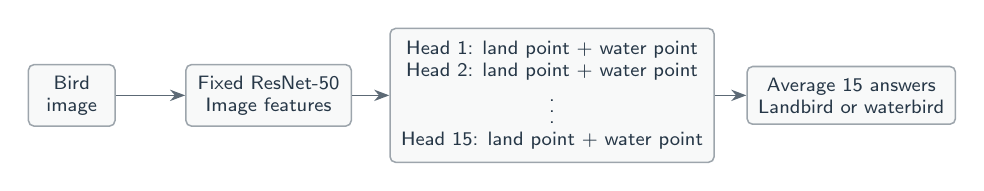
\begin{tikzpicture}[dpe diagram]
  \node[dpe box,minimum width=1.1cm] (image) at (0.5,0) {Bird\\image};
  \node[dpe box,minimum width=2.1cm] (net) at (3,0)
    {Fixed ResNet-50\\Image features};
  \node[dpe box,minimum width=3.2cm,minimum height=1.7cm] (heads) at (6.6,0)
    {Head 1: land point + water point\\Head 2: land point + water point\\$\vdots$\\Head 15: land point + water point};
  \node[dpe box,minimum width=2.1cm] (avg) at (10.4,0)
    {Average 15 answers\\Landbird or waterbird};
  \draw[dpe arrow] (image) -- (net);
  \draw[dpe arrow] (net) -- (heads);
  \draw[dpe arrow] (heads) -- (avg);
\end{tikzpicture}
}
\caption{DPE uses one shared feature extractor and 15 heads. Changing the
head combination changes how the final answers count.}
\label{fig:dpe}
\end{methodfigure}

The gains from our earlier changes were small or depended on the
validation split. We wondered whether the heads were repeating the same
decision rule, or whether the shared features were making some birds
hard to recognize. This week we checked the heads, found recurring
image failures, and tested those birds under a background edit.

\textbf{Models and data.} We used five saved standard ERM models
(seeds 0--4) and two enhanced ERM$^*$ models (seeds 0--1). ERM is ordinary
training. Our enhanced recipe trains for 400 epochs instead of 100
and uses altered versions of the training images. The checks below use
validation images, separate from the images that trained ResNet.

\newpage
\section{From DPE Heads to Recurring Failures}

\subsection{Were the heads learning almost the same rule?}

We first compared the directions that determine each head's decision.
A direction describes which changes in the image features increase
the head's waterbird score. We measured how closely two directions
align using cosine similarity. A value near 1 means they are almost
the same.

There are 105 pairs in each 15-head ensemble, giving 735 pairs across
our seven saved models. Every pair was below 0.90, the least restrictive
cutoff in this check (Table~\ref{tab:heads}). We also checked their
predictions on the same 479 validation images. The heads disagreed
on some images and corrected some of each other's mistakes.

\begin{table}[H]
\centering
\caption{Largest decision-direction similarity in the saved ensembles.
All pairs were below the 0.90 cutoff.}
\label{tab:heads}
\small
\begin{tabular}{@{}lrrr@{}}
\toprule
Training recipe & Models & Head pairs & Largest similarity\\
\midrule
Standard ERM & 5 & 525 & 0.598\\
Enhanced ERM$^*$ & 2 & 210 & 0.741\\
\bottomrule
\end{tabular}
\end{table}

This gave little support for the particular redundancy we had suspected.
We put retraining for that idea on hold and looked at the birds that
kept causing mistakes.

\subsection{Which birds kept failing?}

We fitted linear classifiers on the saved features and recorded their
mistakes across the 1,199 validation images. To score each image,
we fitted its classifier on the other four parts of a five-part
validation split. This lets us inspect predictions for images left
out of that classifier's fit.

We found 26 images that at least four of five standard models got wrong,
while both enhanced models got right (Fig.~\ref{fig:selection}).
Half showed landbirds on water and half showed waterbirds on land.
We also selected 80 birds that all seven models got right in this audit,
with 40 from each of the same two groups.

\begin{methodfigure}
\resizebox{\linewidth}{!}{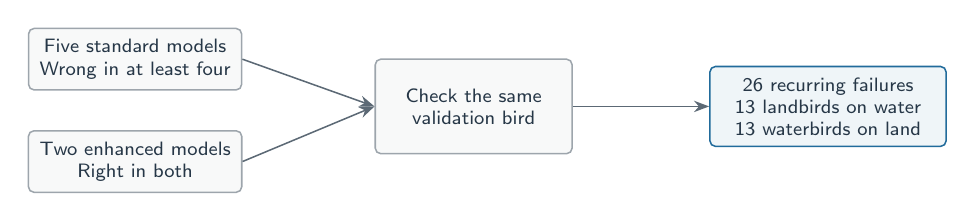
\begin{tikzpicture}[dpe diagram]
\node[dpe box,minimum width=2.4cm] (s) at (1.2,0.6) {Five standard models\\Wrong in at least four};
\node[dpe box,minimum width=2.4cm] (e) at (1.2,-0.7) {Two enhanced models\\Right in both};
\node[dpe box,minimum width=2.5cm,minimum height=1.2cm] (same) at (5.5,0) {Check the same\\validation bird};
\node[dpe box,draw=dpewater,fill=dpewater!7,minimum width=3cm] (keep) at (10,0) {26 recurring failures\\13 landbirds on water\\13 waterbirds on land};
\draw[dpe arrow] (s.east) -- (same.west);
\draw[dpe arrow] (e.east) -- (same.west);
\draw[dpe arrow] (same.east) -- (keep.west);
\end{tikzpicture}
}
\caption{How we selected the recurring failures. The enhanced models
gave us examples of the same birds being classified correctly.}
\label{fig:selection}
\end{methodfigure}

\newpage
\section{Trying Different Final Classifiers}

Before changing the image, we checked whether a different final
classifier could recognize more of the 26 birds. Deep Feature
Reweighting (DFR) retrains a linear classifier on saved features.
A linear classifier gives each feature a weight and adds the results
to make a prediction.

We also tried classifiers that can learn more complicated rules,
including a small neural network (MLP) and a radial-basis support
vector machine (RBF-SVM). The comparison kept ResNet fixed.
Each image was scored by a classifier fitted on other validation images.

\begin{methodfigure}
\resizebox{\linewidth}{!}{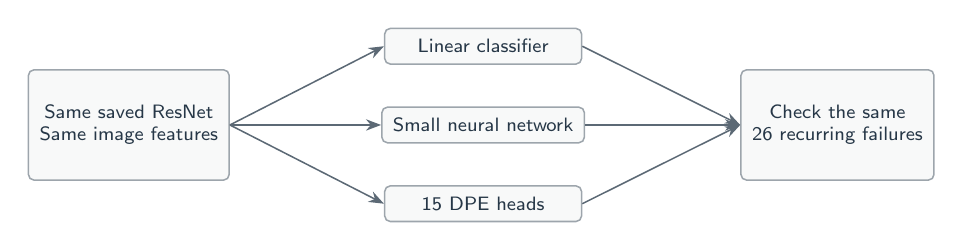
\begin{tikzpicture}[dpe diagram]
\node[dpe box,minimum height=1.4cm] (fixed) at (1.5,0)
 {Same saved ResNet\\Same image features};
\node[dpe box,minimum width=2.5cm] (linear) at (6,1) {Linear classifier};
\node[dpe box,minimum width=2.5cm] (mlp) at (6,0) {Small neural network};
\node[dpe box,minimum width=2.5cm] (dpe) at (6,-1) {15 DPE heads};
\node[dpe box,minimum height=1.4cm] (check) at (10.5,0)
 {Check the same\\26 recurring failures};
\foreach \head in {linear,mlp,dpe}{
 \draw[dpe arrow] (fixed.east) -- (\head.west);
 \draw[dpe arrow] (\head.east) -- (check.west);
}
\end{tikzpicture}
}
\caption{Change the final classifier while keeping its input features
fixed. The table also includes the RBF-SVM comparison.}
\label{fig:readouts}
\end{methodfigure}

\begin{table}[H]
\centering
\caption{Share of the 26 selected failures classified correctly in
the saved classifier checks, averaged over five standard models.}
\label{tab:readouts}
\small
\begin{tabular}{@{}lr@{}}
\toprule
Final classifier & Correct (\%)\\
\midrule
Linear classifier (DFR-L2) & 4.6\\
RBF-SVM & 33.9\\
Small neural network (MLP) & 36.9\\
15-head DPE & 43.9\\
\bottomrule
\end{tabular}
\end{table}

The more flexible classifiers recovered some birds, but still missed
over half of this selected set. This made us ask whether the background
was affecting the features before they reached the classifier.

A separate check allowed small internal scale and shift parameters
inside ResNet to change, along with the final classifier. This
\emph{Affine-DFR} check reached 63.1\% on the same selected failures.
It gave us another reason to inspect the feature extractor. We then
used the supplied bird outlines to check which spatial cells the
classifier was reading.

\newpage
\section{Giving the Bird More Weight}

A ResNet-50 produces a $7\times7$ grid for a $224\times224$ image.
Each of the 49 cells contains 2,048 feature values. Usually the model
averages all cells equally, so cells covering mostly scenery count
as much as cells covering mostly bird.

We tried giving more weight to the bird's location. The original CUB
dataset supplies a \emph{mask}, a map marking the bird's outline.
We resized and cropped it with the image, then averaged it down to
$7\times7$. A cell receives more weight when more of its corresponding
image area is covered by the bird.

\begin{methodfigure}
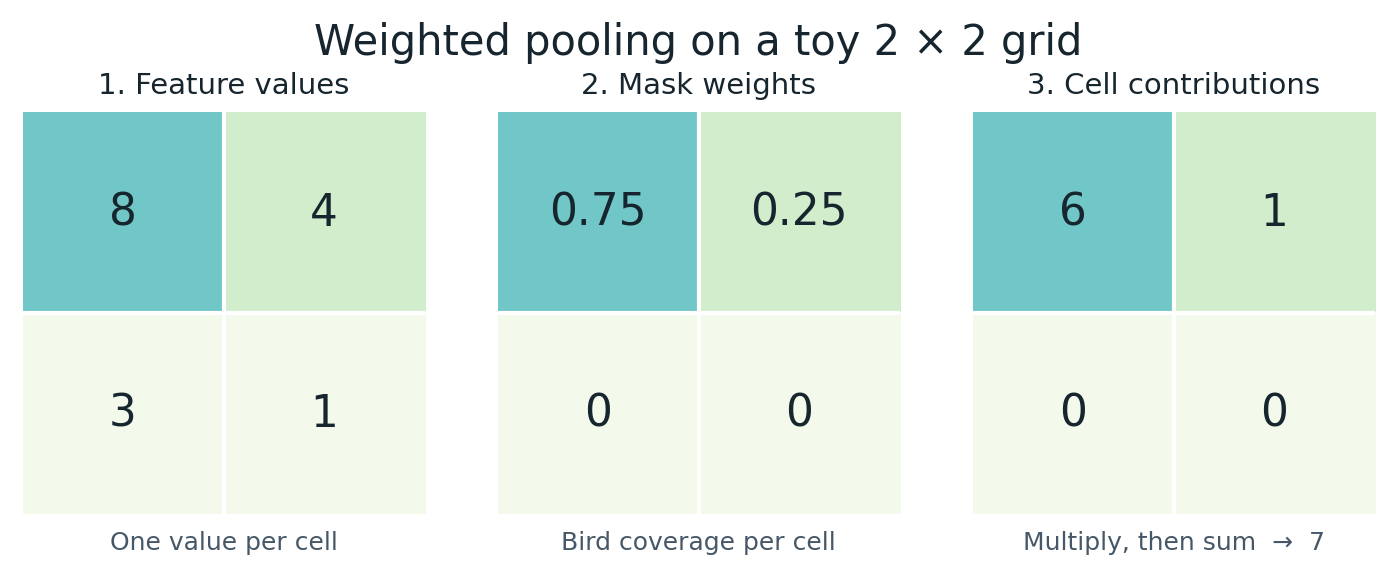
\includegraphics[width=0.95\linewidth]{figures/weighted_grid.png}
\caption{A four-cell example. Multiply each feature value by its weight,
add the results, and divide by the sum of the weights. Here the weights
sum to 1, so the result is $8\times0.75+4\times0.25=7$.}
\label{fig:weights}
\end{methodfigure}

We fitted a new linear classifier on these weighted features. This
follows the idea behind Deep Feature Reweighting, which retrains a
model's final classifier on fixed features. Our added check changes
which spatial cells contribute to those features.

There was still a reason the background might matter. ResNet processes
the whole image before we apply the mask weights. As it combines
neighboring locations, a cell over the bird can also pick up information
from the scene. We therefore compared the same bird before and after
replacing its background.

\begin{methodfigure}
\resizebox{\linewidth}{!}{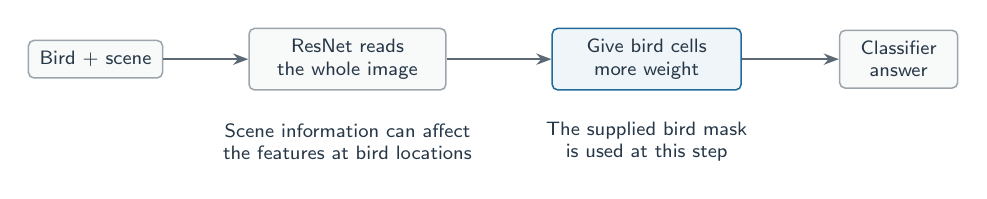
\begin{tikzpicture}[dpe diagram]
\node[dpe box,minimum width=1.5cm] (im) at (0.8,0) {Bird + scene};
\node[dpe box,minimum width=2.5cm] (net) at (4,0) {ResNet reads\\the whole image};
\node[dpe box,draw=dpewater,fill=dpewater!7,minimum width=2.4cm] (pool) at (7.8,0) {Give bird cells\\more weight};
\node[dpe box,minimum width=1.5cm] (out) at (11,0) {Classifier\\answer};
\draw[dpe arrow] (im) -- (net);
\draw[dpe arrow] (net) -- (pool);
\draw[dpe arrow] (pool) -- (out);
\node[align=center,text width=3.5cm] at (4,-1.05) {Scene information can affect\\the features at bird locations};
\node[align=center,text width=3.5cm] at (7.8,-1.05) {The supplied bird mask\\is used at this step};
\end{tikzpicture}
}
\caption{Where the mask is used. Giving a bird cell more weight can
retain scene information already present in that cell's features.}
\label{fig:pooling}
\end{methodfigure}

\newpage
\section{Changing the Background}

We kept each bird in place and replaced the scene with the same uniform
gray fill. The bird's interior pixels stayed the same, while the mask
blended colors along its outline. Within each original/edited pair,
the ResNet model, mask weights and final classifier stayed fixed.
The classifier had been fitted using other validation images.

For the Parakeet Auklet below, the seed-0 model's waterbird score rose
from 3.5\% to 65.6\%. The score crossed the 50\% cutoff, changing the
answer from landbird to waterbird.

\begin{methodfigure}
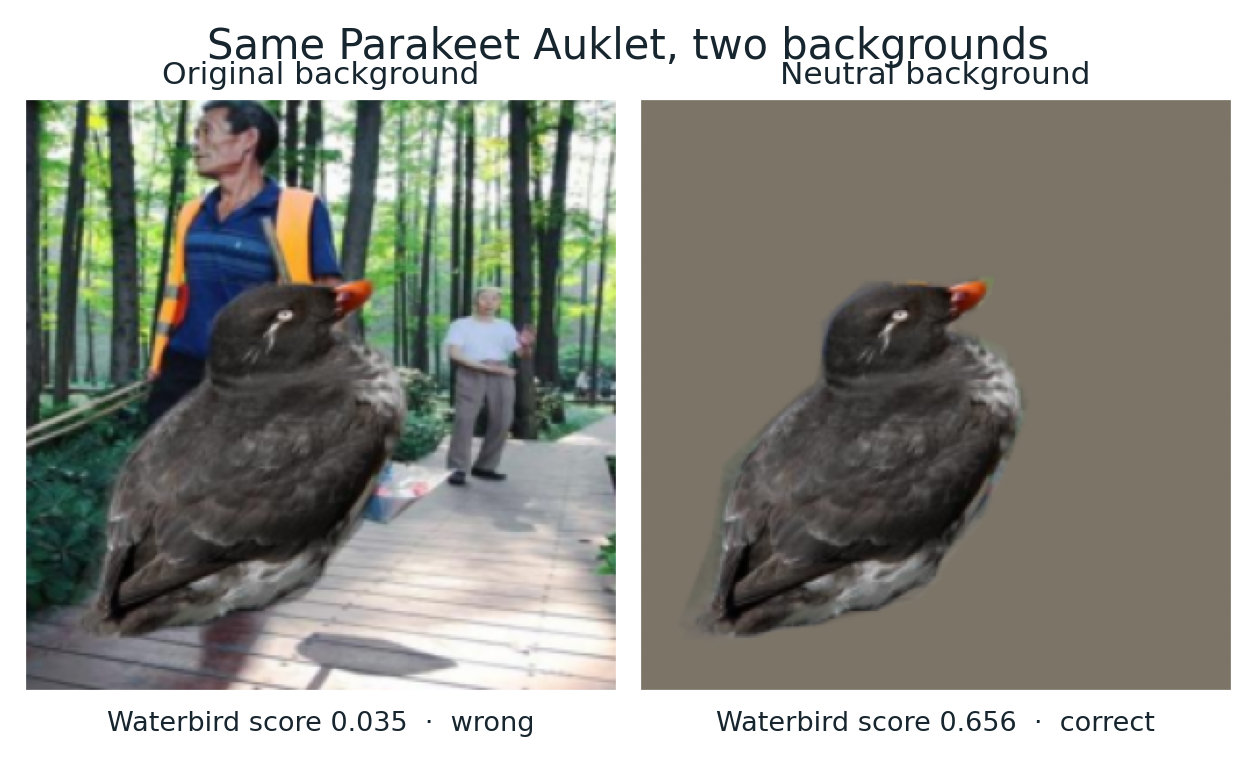
\includegraphics[width=0.8\linewidth]{figures/auklet_pair.png}
\caption{One recurring failure. The bird is a waterbird. Both predictions
use the same model and mask weighting.}
\label{fig:auklet}
\end{methodfigure}

\textbf{Results.} We tested all 26 birds with each of the five standard
models, giving 130 paired evaluations. Correct predictions rose from
53 to 106. Fifty-four answers went from wrong to right, and one went
from right to wrong. Both bird/background groups improved
(Table~\ref{tab:edit}).

\begin{table}[H]
\centering
\caption{Accuracy (\%) with mask weighting. Each bird is evaluated by
five models. The two group rows break down the 26 failures.}
\label{tab:edit}
\small
\begin{tabular}{@{}lrrr@{}}
\toprule
Selected images & Birds & Original & Gray fill\\
\midrule
Recurring failures & 26 & 40.8 & 81.5\\
\quad Landbirds on water & 13 & 46.2 & 83.1\\
\quad Waterbirds on land & 13 & 35.4 & 80.0\\
\midrule
Passing comparison set & 80 & 98.0 & 96.3\\
\bottomrule
\end{tabular}
\end{table}

\newpage
\section{Checking What Changed}

All five standard models improved on the selected failures. The edit
had a different effect on the 80 birds that had passed the earlier
audit. With mask weighting, their correct predictions fell from
392/400 to 385/400. This comparison helped us see that the large
recovery was concentrated in the selected failure set.

We then checked the features at the bird's location inside ResNet.
At each of its four main stages, we compared a mask-weighted feature
vector for the original image with one for the edited image.
We call their relative difference \emph{feature drift}. Zero means
the two vectors are identical. Higher values mean a larger change.

\begin{methodfigure}
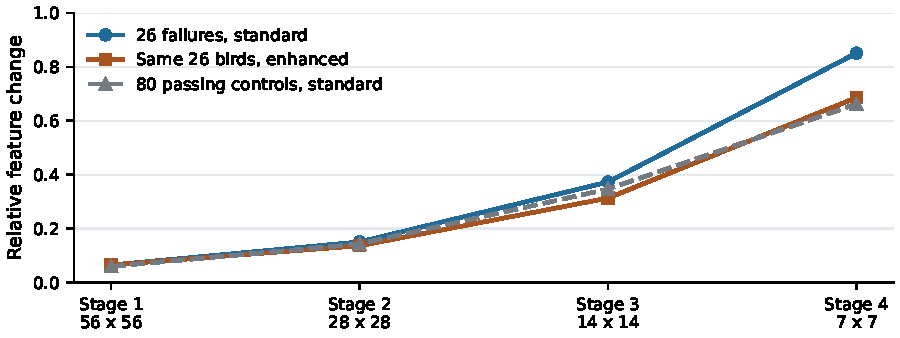
\includegraphics[width=0.96\linewidth]{figures/week04_feature_drift.pdf}
\caption{Feature drift after the gray edit. Each value summarizes
features weighted by the bird mask. The difference is scaled by the
average length of the original and edited feature vectors.}
\label{fig:drift}
\end{methodfigure}

The change grew across the four stages. At the final stage it reached
0.851 for the standard models on the recurring failures, compared with
0.686 for the enhanced models on the same birds. The passing comparison
set also showed drift, although the standard models' final value was
lower at 0.662. These measurements are consistent with the scene
affecting features at the bird's location.

\textbf{What we take from this.} Giving the bird's location more weight
helped, but many predictions still depended on the background edit.
This moved our attention from combining final answers toward how
the network builds its features before the weighted average.

The 26 birds were selected for earlier mistakes, and all five models
saw the same birds. The edit also changes contrast and blends boundary
pixels. The result describes sensitivity to this edit on these
selected validation examples.

\paragraph{Run notes.}
Classifier fits used our previously corrected labels. The selected
birds exclude the three relabeled species. Detailed settings and
outputs are in the
\evidence{results/dpe/head_diversity_20261122/README.md}{DPE pilot},
\evidence{results/rep_repair/phase_a_20261123/README.md}{classifier checks},
\evidence{results/rep_repair/phase_b_controls_20261123/README.md}{internal scaling check}
and \evidence{results/rep_repair/phase_b_counterfactuals_20261123/README.md}{background-edit records}.
The final-classifier approach follows
\href{https://arxiv.org/abs/2204.02937}{Deep Feature Reweighting}.

\end{document}
